\documentclass[12pt]{article}
\usepackage[a4paper]{}
\usepackage{graphicx}
\usepackage[utf8]{inputenc}
\usepackage{amsmath}
\usepackage[]{algorithm2e}
\usepackage{comment}
\usepackage{soul}
\usepackage{cancel}
\usepackage{multirow}
\usepackage{chngcntr}
\usepackage{enumitem}
\usepackage{booktabs}
\usepackage[table,xcdraw]{xcolor}
\counterwithin{table}{section}
\usepackage{subfigure}
\usepackage{array}
\usepackage{float}
\restylefloat{table}
\graphicspath{ {images/} }
%\topmargin 15mm
\numberwithin{figure}{section}
\providecommand{\keywords}[1]{\textbf{\textit{Keywords---}} #1}
\headheight 10pt
\oddsidemargin 0mm
%\evensidemargin -5mm
\textwidth 161mm
\textheight 210mm
\linespread{1.3}
\begin{document}
\thispagestyle{empty}
 \begin{center}
Major Project Proposal Report\\
\null
on\\
\null
\textbf{Automatic Generation of Medical Imaging Reports}\\
\null
Submitted by \\
\null
\textbf{Rahul Kumar}\\
\textbf{172IT014}\\
\textbf{M.Tech (IT)}\\
\null
Under the Guidance of\\
\textbf{Dr. Sownmya Kamath S.}  \\
\null
\textbf{Dept. of Information Technology,}\\
\textbf{NITK, Surathkal}\\
\null
\textbf{Date of Submission: 18-10-2018}\\
\begin{figure}[h] % b - bottom, t - top, h - here
 \centering{
 
\includegraphics[scale=0.7]{logo.jpg}
 }
\end{figure}
\textbf{Department of Information Technology\\
National Institute of Technology Karnataka, Surathkal\\
2018-2019}\\
\end{center}
\clearpage
\thispagestyle{empty}
\begin{center}
\underline{\textbf{CERTIFICATE}} \\
\end{center}
\null
This is to certify that the major project entitled "Automatic Generation of Medical Imaging Reports" is a bonafide work carried out as part of the course Major Project (IT898), under my guidance by Rahul Kumar, student of III Semester M.Tech (IT) at the Department of Information Technology, National Institute of Technology Karnataka, Surathkal, during the academic semester Jul - Nov 2018, in partial fulfillment of the requirements for the award of the degree of Master of Technology in Information Technology, at NITK Surathkal. 
\\
\\
\\
\\
\\
\\
\begin{minipage}{0.4\textwidth}
\begin{flushleft}
Signature of the Student\\
Place: Mangalore\\ 
Date:28-09-2018\\
\end{flushleft}
\end{minipage}
\begin{minipage}{0.4\textwidth}
\begin{flushright}
Signature of the Instructor(s)\\
\end{flushright}
\end{minipage}
\\
\\
\\
\clearpage
\thispagestyle{empty}
\begin{center}
\underline{\textbf{DECLARATION}}\\
\end{center}
\null
I hereby declare that the Major Project entitled “Automatic Generation of Medical Imaging Reports” submitted as part of the partial course requirements for the course Major Project (IT898) , for the award of the degree of Master of Technology in Information Technology at NITK Surathkal during the Jul - Nov 2018 semester, has been carried out by me. I declare that the project has not formed the basis for the award of any degree, associate ship, fellowship or any other similar titles elsewhere.\\ 
\\
\\
\\
\\
\\
\\
Signature of the Student\\
Place: Mangalore\\
Date:28-09-2018\\
\clearpage
\pagenumbering{roman}
\section*{Abstract}
Apart from being an interesting computer-vision problem, manual analysis of radiology images also needs to be performed by experienced radiologist which makes this issue even more necessary to be addressed. Automatic description generation for radiology images can benefit radiologist with quick, localised and explanatory analysis. Expected analysis must contain keywords (Tags) that images relates with, observation for different body parts in the image ( Findings), and the diagnosis ( Impression ).
Our goal here is comprises of three tasks, to classify given X-ray image against list of medical abnormalities resulting in tagged images, to generate narration along with localising region for found abnormalities, and finally using hierarchical LSTM, generating long report description .
We are 

\\
Keywords - Machine learning, GAN, deep learning, neural nets, DCGAN.
\\
\clearpage
\tableofcontents
\clearpage
\listoffigures 
\listoftables
\clearpage
\pagenumbering{arabic}
\section{Introduction}
\paragraph{Medical images : }
Radiologist analyze and diagnose using medical images for various diseases on a daily basis. However analysis, reading and interpretation, and writing textual report demands skills such as knowledge of anatomy and basic details about the visual symptoms of the disease, knowledge of correlation with other diagnostic results like pathology result etc.
Writing diagnostic report for radiology image, even for experienced radiologists is a time consuming process. And this same task sometimes is required to be repeated for up to hundreds of different radiology images everyday.
\paragraph{Medical reporting task and parts of report : }
Medical reporting procedure for radiology images include radiologist analyzing various part of patient’s body and remarking various findings about those body parts. Sometimes different related or unrelated findings about different body parts can be observed in single images. Those findings and other observation then lead to a further consolidated overall diagnostic report about the patient known as Impression. In this process images needs to be given proper tags for future categorization and quick analysis purpose.
\paragraph{}
So our challenge is to provide solution for generating tags, findings and impression for a given radiology image. As the process of diagnostic, our challenge is can be broken down in three stages, starting with tags generation for a given image. We are solving this problem by classifying the images against various pre-known labels and thus solving it as a multi-label classification problem. Tags generated at this step are preserved for future query purpose as well as as input for further processing of images. 
\paragraph{}
We will be using Generative adversarial networks for multi-label classification. For our task, we setup a GAN for generating new sample data for N classes and then classifying it for N+1 classes, representing N real classes for N labels and one class for fake data.
Various regions of an image may contain different information for different body parts, which can be related sometimes or to be looked as unrelated multiple diagnostic many other times. This task includes localising the image regions and then generating narration for those regions. We are using a co-attention mechanism for analysing given images and the tags generated in multi-label classification process for the given image simultaneously and provide semantic information which can be used for further processing along with previously generated tags information.
\paragraph{}
Generating paragraph of description using hierarchical LSTM
Our third task is to generate descriptions for imaging report summarizing the findings for various regions of images. Description are usually long paragraphs having multiple lines. So this task presents challenges as generating long paragraphs is a nontrivial task. We will be using hierarchical LSTM\cite{2} with co-attention mechanism for generating findings for various regions and then combining them and further processing for description summary generation.
\paragraph{}
To summarize, our multi-task learning framework  will be generating tags, sentences for findings and multi-sentence textual description for given radiology images.


\clearpage


\section{Literature Survey}
\subsection{Background Study}
\paragraph{}
Generating text label for images has been addressed as a multi-label classification task in many previous research. My base paper used pre-trained vgg19 model to classify x-ray images for various class by extracting features from last convolution layer and last two fully connected layers of vgg-19 as multi-label classifier. vgg-19 is trained on a stack of convolutional-maxpooling layer followed by fully connected layers. Max-pooling causes loss of important spatial information and it makes the network ignore the relation between the part and the whole image.


\paragraph{}
Most recent image captioning models are based on a CNN-RNN framework (\cite{4};Karpathy and Fei-Fei, 2015\cite{5}; Krause et al., 2017\cite{6}). Recently, attention mechanisms have been shown to be useful for image captioning (Xu et al., 2015\cite{7}; You et al., 2016\cite{8}). Xu et al. (2015)\cite{7} introduce a spatial-visual attention mechanism over image features extracted from intermediate layers of the CNN. You et al. (2016)\cite{8} propose a semantic attention mechanism over tags of given images. Rather than adopting a single-layer LSTM (Hochreiter and Schmidhuber, 1997)\cite{11}, which is less capable of modeling long word sequences, we leverage the compositional nature of the report and the visual features along with semantic tags, we adopt  a hierarchical LSTM for paragraph generation with a co-attention network to generate topics. 
\paragraph{}
Recent work on GAN (Goodfellow
et al., 2014)\cite{9} have achieved stable to train GANS such as DCGAN \cite{10} building good image representations by training Generative Adversarial Networks (GANs) and later reusing parts of the generator and discriminator networks as feature extractors for supervised tasks. 
\paragraph{}


\clearpage
\subsection{Outcome of Literature Survey}

\begin{table}[H]
\caption{Outcome of Literature Survey}
\label{Outcome of Literature Survey}
\centering
\resizebox{\textwidth}{!}{%
\begin{tabular}{|c|c|c|c|}
\hline
\rowcolor[HTML]{C0C0C0} 
\textbf{Authors} & \textbf{Method} & \textbf{Advantages} & \textbf{Limitations} \\ \hline
Zhang et al., 2017 & \begin{tabular}[c]{@{}c@{}} generating \\semi-structured\\ pathology reports\\using LSTM & CNN\end{tabular} & \begin{tabular}[c]{@{}c@{}}Attention based.\end{tabular} & \begin{tabular}[c]{@{}c@{}}Contents are\\restricted to\\5 predefined topics.\end{tabular} \\ \hline
\begin{tabular}[c]{@{}c@{}}Liang et al.\end{tabular} & \begin{tabular}[c]{@{}c@{}}Recurrent\\topic-transition GAN\\for visual paragraph\\generation\end{tabular} & \begin{tabular}[c]{@{}c@{}}Uses\\Hierarchical LSTM for \\sentance generation.\end{tabular} & \begin{tabular}[c]{@{}c@{}}No Co-attention\\ mechanism.\end{tabular} \\ \hline
\begin{tabular}[c]{@{}c@{}}Radford et. al.\end{tabular} & \begin{tabular}[c]{@{}c@{}}GAN using all\\Deep convolution\\ net without pooling\\\end{tabular} & \begin{tabular}[c]{@{}c@{}}Stable to train,\\ Discriminator can\\serve as classifier \end{tabular} & \begin{tabular}[c]{@{}c@{}}used for image generation.\end{tabular} \\ \hline
\begin{tabular}[c]{@{}c@{}}Visual Geometry Group\end{tabular} & \begin{tabular}[c]{@{}c@{}}VGG 19\\convolution+pooling\\based pretrained model\end{tabular} & \begin{tabular}[c]{@{}c@{}}Pretrained for\\1000 classes\\Free to use\end{tabular} & \begin{tabular}[c]{@{}c@{}}Maxpooling cause spatial information loss.\end{tabular} \\ \hline
\end{tabular}
}
\end{table}
\paragraph{}
Many researchers have explored various convolution based architectures for Multi-label classification and RNN-CNN based  text generation for images, but recent developments in GAN architecture provides a new approach to learn better image representations.  
 \subsection{Problem Statement}
 \paragraph{}
 Using GANs to improve multi-label classification efficiency for “Tag generation task” in Automatic Generation of natural Medical Imaging Reports
\subsection{Objectives}
\begin{itemize}
\item Generating Sample using various GAN architectures.
\item Building GAN based classifier.
\item Training of deep learning network architectures.
\item Post processing of the results to optimize the results.
\item implementation of real-life application for proposed architecture
\end{itemize}
\clearpage
\section{Research Methodology and Materials}
\subsection{Datasets}
\paragraph{}
Our training dataset will be a collection of X-ray images and atgs, findings and impressions along with each X-ray images 
\subsection{Proposed Methodology}
Overview
We are proposing a multi-task framework to perform both tag prediction and description generation for given x-ray image. For a given input X-ray image, our framework will generate long natural reports covering diverse topic.  
\paragraph{}


\begin{figure}[h]
    \centering
    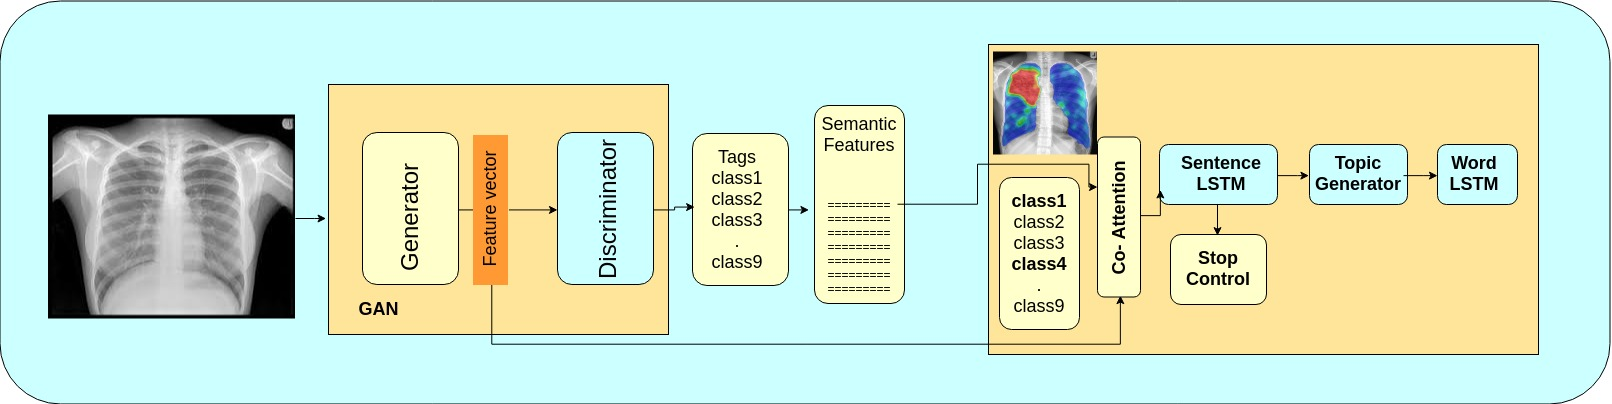
\includegraphics[width=\textwidth]{framwork.jpg}}
    \caption{Framework for automatic description generator}
    \label{fig:my_label}
\end{figure}
\subsubsection{Tag prediction}

One X-ray image can have more than one abnormalities. Predicting tags will require classifying each image against various classes of abnormalities, hence a multi-class classifier suits our need best. We will use a Deep Convolution GAN (DCGAN)\cite{3}, a variation of GAN. Dsicriminator of train DCGAN will  be used for semi-supervised learning for multi-label classification of images and as well as for extracting feature vector to be used by co-attention mechanism later. For classifying for multiple label we will use softmax layer on outmost fully connected layer instead of sigmoid, giving us probability for image belonging to N classes. Last convolution layer from discriminator architecture will give us feature vector.
\begin{figure}[h]
    \centering
    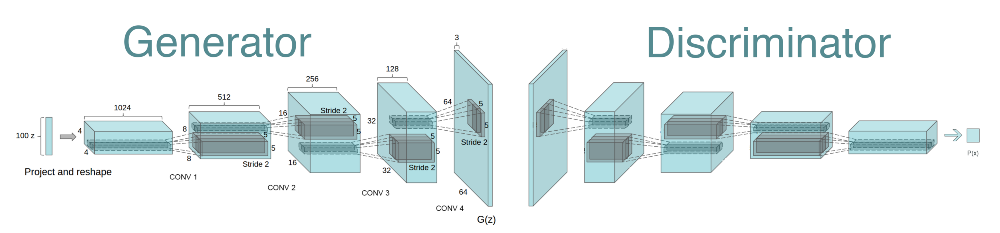
\includegraphics[width=\textwidth]{dcgan.png}
    \caption{Architecture for DCGAN. Notice there are no Spatial Pooling layer.}
    \label{fig:my_label}
\end{figure}
\paragraph{}
\begin{figure}[h]
    \centering
    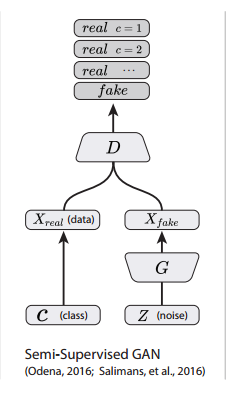
\includegraphics[width=130]{ACGAN.png}
    \caption{Architecture for CatGAN. Here Real images from different classes are used to train with generator generating new images for that particular classes.}
    \label{fig:my_label}
\end{figure}
\paragraph{}
\subsubsection{Co-attention}
The previous step added tags to our information and now for utilizing both visual information of a region of the image and predicted tags. We are utilising co-attention mechanism to simultaneously attend to both modalities.
Joint context vector is generated using embedding vector for most likely tags, feature vector from MLC, combined with previous hidden state of Sentence LSTM generating soft semanntic attentions and soft visual attentions over given image features and tags. Further visual and semantic context vecotr, produced separately will be combined by concatenating.
Visual and semantic context vectors will be computed
\paragraph{}
\subsubsection{Hierarchica LSTM}
Here Network hierarchically builds an embedding for a paragraph from embeddings for sentences and words, then decodes this embedding to reconstruct the paragraph
{Sentence LSTM} will be single layer LSTM using joint context vector as its input generates topic vector for word LSTM, next level of hierarchical LSTM using topic generator combined with stop control mechanism.
Word LSTM Taking the topic vector and START token as inital input 
\paragraph{}

\section{Conclusion and Future Work}
\paragraph{}
Learning better image  representation can help us developing better classifier ( discriminator architecture) and using GAN also allow us to explore the idea of generating new image samples for further learning and for applications like generating full x-ray from incomplete or generating image for lateral view from front view X-ray or vice-versa. 
\paragraph{}
Another way to improve the framework is to use GANs with Self -Attention capabilities.
\clearpage
\section{Time line of the project}
\begin{table}[htp]
\centering
\caption{Time line for completion of project}
\label{my-label}
\begin{tabular}{|
>{\columncolor[HTML]{EFEFEF}}l |l|l|l|l|l|l|l|}
\hline
\cellcolor[HTML]{CBCEFB}\textbf{Milestone} &                                      &                                &                                &        &                                &                                &                                  \\ \hline
Feasibility Study                          & \cellcolor[HTML]{C0C0C0}Jul-Sep 2018 &            &                          &                                &                                &                                &                                    \\ \hline
Objective 1                     &                                                      & \cellcolor[HTML]{C0C0C0}Oct 18 &            &                    &                                &                                &                                    \\ \hline
Objective 2                      &                                                &                                & \cellcolor[HTML]{C0C0C0}Nov 14 &     &                           &                                &                                    \\ \hline
Objective 3                &                                                      &                                &                                & \cellcolor[HTML]{C0C0C0}Dec 18 &      &                          &                                    \\ \hline
Objective 4                    &            &                                      &                                &                                & \cellcolor[HTML]{C0C0C0}Dec 18 &                                &                                    \\ \hline
Objective 5                      &          &                                      &                                &                                &                                & \cellcolor[HTML]{C0C0C0}Jan 20 &                                    \\ \hline
Final Submission                   &        &                                      &                                &                                &                                &                                & \cellcolor[HTML]{C0C0C0}Jan 20 - May 19 \\ \hline
\end{tabular}
\end{table}
\clearpage
\addcontentsline{toc}{section}{References}
\begin{thebibliography}{}
\bibitem{1}
Jing, Baoyu, Pengtao Xie, and Eric Xing. "On the automatic generation of medical imaging reports." arXiv preprint arXiv:1711.08195 (2017).
\bibitem{2}
Krause, Jonathan, et al. "A hierarchical approach for generating descriptive image paragraphs." Computer Vision and Pattern Recognition (CVPR), 2017 IEEE Conference on. IEEE, 2017.

\bibitem{3}
Suárez, Patricia L., Angel D. Sappa, and Boris X. Vintimilla. "Infrared image colorization based on a triplet DCGAN architecture." Computer Vision and Pattern Recognition Workshops (CVPRW), 2017 IEEE Conference on. IEEE, 2017.
 \bibitem{4}
 Oriol Vinyals, Alexander Toshev, Samy Bengio, and
Dumitru Erhan. Show and tell: A neural image
caption generator. In Proceedings of the IEEE conference
on computer vision and pattern recognition,
pages 3156–3164, 2015.
\bibitem{5}
Karpathy, Andrej, and Li Fei-Fei. "Deep visual-semantic alignments for generating image descriptions." Proceedings of the IEEE conference on computer vision and pattern recognition. 2015.
\bibitem{6}
Krause, Jonathan, et al. "A hierarchical approach for generating descriptive image paragraphs." Computer Vision and Pattern Recognition (CVPR), 2017 IEEE Conference on. IEEE, 2017.
\bibitem{7}
Xu, Kelvin, et al. "Show, attend and tell: Neural image caption generation with visual attention." International conference on machine learning. 2015.
\bibitem{8}
You, Quanzeng, et al. "Image captioning with semantic attention." Proceedings of the IEEE conference on computer vision and pattern recognition. 2016.
\bibitem{9}
Goodfellow, Ian, et al. "Generative adversarial nets." Advances in neural information processing systems. 2014.
\bibitem{10}
Radford, Alec, Luke Metz, and Soumith Chintala. "Unsupervised representation learning with deep convolutional generative adversarial networks." arXiv preprint arXiv:1511.06434 (2015).
\bibitem{11}
Hochreiter, Sepp, and Jürgen Schmidhuber. "Long short-term memory." Neural computation 9.8 (1997): 1735-1780.
\bibitem{12}
Liang, Xiaodan, et al. "Recurrent topic-transition GAN for visual paragraph generation." arXiv preprint arXiv:1703.07022 (2017).
\end{thebibliography}

\end{document}